% From: https://texample.net/tikz/examples/complete-graph/
\documentclass{standalone}
\usepackage{tikz}
\usetikzlibrary[topaths]
\begin{document}
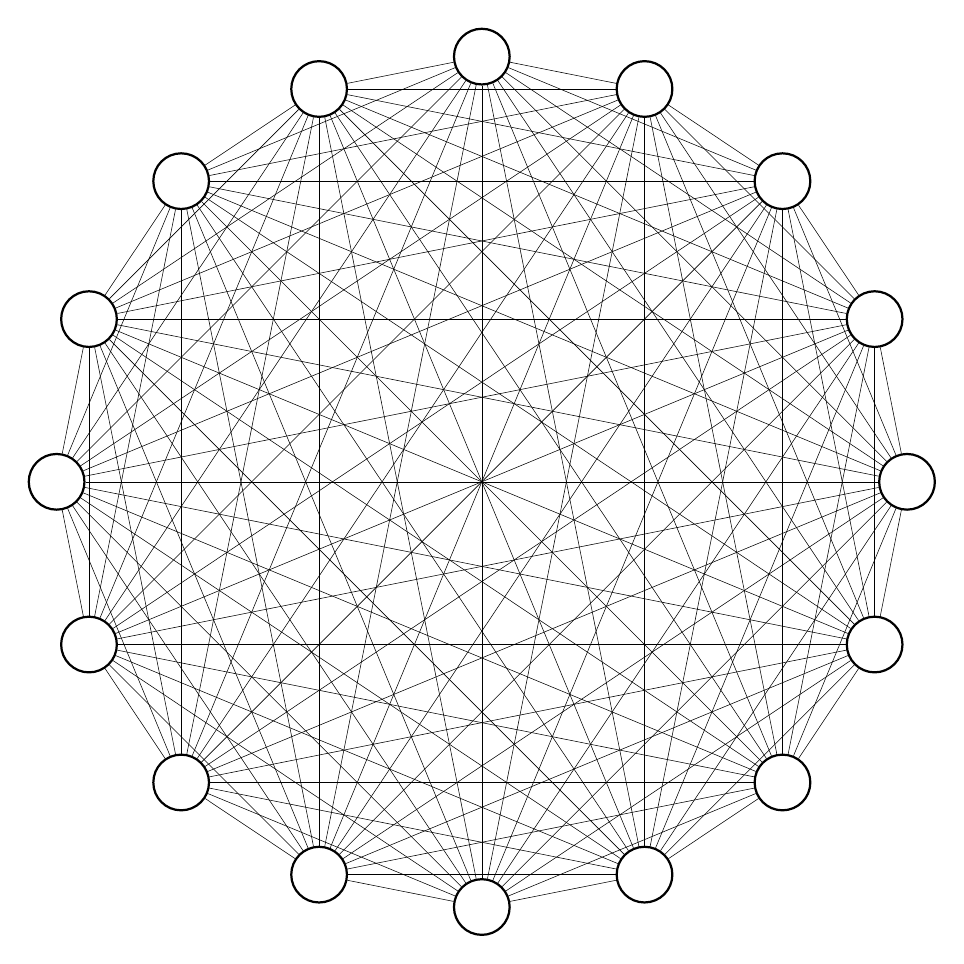
\begin{tikzpicture}[transform shape,line width=0.2pt]
  \foreach \x in {1,...,16}{%
    \pgfmathparse{(\x-1)*45+floor(\x/9)*22.5}
    \node[draw,circle,inner sep=0.25cm] (N-\x) at (\pgfmathresult:5.4cm) [thick] {};
  }
  \foreach \x [count=\xi from 1] in {2,...,16}{%
    \foreach \y in {\x,...,16}{%
        \path (N-\xi) edge[-] (N-\y);
  }
}
\end{tikzpicture}
\end{document}
